\documentclass[autodetect-engine,dvipdfmx-if-dvi,ja=standard,a4j,jbase=11pt,magstyle=nomag*]{bxjsreport}
% \documentclass[uplatex, dvipdfmx, a4paper, 11ptj, report]{jsbook}
% small japanese font size:     9pt, 10pt, 11pt, 12pt, 14pt, ... (please refer the document of jsclasses)
% word-like japanese font size: 10ptj 10.5ptj, 11ptj, 12ptj (or jbase=xxpt (without 'j') if error is occured)

\usepackage{ifptex,ifxetex,ifluatex}
\ifluatex
    \usepackage{bxcalcux}
    \ltjsetparameter{jacharrange={-2,-3}}
    \usepackage{luatexja-otf}
    \usepackage{bxbase}
\else\ifxetex
    % \usepackage{zxjatype}
    % \usepackage[macros]{zxotf}
    \XeTeXgenerateactualtext=1
    \usepackage{xltxtra}
    \usepackage{bxbase}
\else\ifuptex
    \usepackage{otf}
    \usepackage[prefernoncjk]{pxcjkcat}
    \cjkcategory{sym11,sym18,sym19}{cjk}
    \usepackage[utf8]{inputenc}
    \usepackage{pxbase}
\else\ifstrictptex
    \usepackage{otf}
    \usepackage[utf8]{inputenc}
    \usepackage{pxbase}
\fi\fi\fi\fi

\usepackage[LGR,T2A,T1]{fontenc}

\usepackage{graphicx}
% \usepackage[dvipdfmx]{graphicx}
\usepackage{grffile}

% paper layout setting
\setpagelayout{noheadfoot, left=18.0truemm, right=18.0truemm, top=29.0truemm, bottom=26.0truemm, columnsep=6.5truemm}
% \setpagelayout{noheadfoot, left=15.0truemm, right=5.0truemm, top=12.5truemm, bottom=12.5truemm, columnsep=5.0truemm}

% font setting
\usepackage{amsmath}
\usepackage{amssymb}
\usepackage{mathtools}
\usepackage{bm}
\usepackage{fix-cm}
\usepackage{newtxtext}
\usepackage[slantedGreek]{newtxmath}

% caption setting
\usepackage[font=bf,labelfont=bf,labelsep=quad]{caption}

% to balance the last page of the two-column article
% \usepackage[nospread, keeplastbox, nodebug]{flushend}

% title font style
\renewcommand{\headfont}{\bfseries}

% section setting (using titlesec, uelm package)
\renewcommand{\thesection}{\arabic{section}}
\renewcommand{\thesubsection}{\arabic{section}.\arabic{subsection}}

\usepackage[explicit]{titlesec}
\usepackage[normalem]{ulem}
\titleformat{name=\section}{\normalfont\headfont\normalsize\raggedright}{}{0pt}{\uline{\thesection.\quad#1}}
\titleformat{name=\section,numberless}{\normalfont\headfont\normalsize\raggedright}{}{0pt}{\uline{#1}}
% \titleformat{name=\section}{\normalfont\headfont\normalsize\raggedright}{}{0pt}{\thesection.\quad#1}
\titlespacing{name=\section}{0pt}{.5\Cvs plus .0\Cvs minus .3\Cvs}{.1\Cvs plus .0\Cvs minus .1\Cvs}
\titleformat{name=\subsection}{\normalfont\headfont\normalsize\raggedright}{}{0pt}{\thesubsection.\quad#1}
\titleformat{name=\subsection,numberless}{\normalfont\headfont\normalsize\raggedright}{}{0pt}{#1}
\titlespacing{name=\subsection}{0pt}{.3\Cvs plus .0\Cvs minus .2\Cvs}{.0\Cvs plus .0\Cvs minus .0\Cvs}

% \makeatletter
% \renewcommand{\section}{\@startsection{section}{1}{\z@}{.5\baselineskip}{.1\baselineskip}{\normalfont\normalsize\headfont\raggedright}}
% \renewcommand{\subsection}{\@startsection{subsection}{2}{\z@}{.3\baselineskip}{\z@}{\normalfont\normalsize\headfont\raggedright}}
% \makeatother

\usepackage{secdot}
\sectiondot{section}
\sectiondot{subsection}

% list (itemize, enumerate, description, ...)
\usepackage{enumitem}
\setlist[1]{parsep=.0\baselineskip,topsep=.2\baselineskip,itemsep=.1\baselineskip}
% \makeatletter
% \def\@listi{\leftmargin\leftmargini
%     \parsep \z@
%     \topsep .2\baselineskip
%     \itemsep .1\baselineskip \relax}
% \let\@listI\@listi
% \makeatother

% no page number
\pagestyle{empty}

% footnote
\usepackage[bottom,hang,stable]{footmisc}
\setlength{\footnotemargin}{0pt}

% float setting (figure, table)
\setlength\floatsep{2.0truemm}
\setlength\textfloatsep{2.0truemm}
\setlength\intextsep{1.0truemm}
\setlength\dblfloatsep{2.0truemm}
\setlength\dbltextfloatsep{2.0truemm}
\setlength\abovecaptionskip{0.5truemm}
\setlength\belowcaptionskip{0.5truemm}

% lineskip setting (body text, display-style equation)
\AtBeginDocument{%
    \narrowbaselines    % basic english lineskip (for article)
    % \widebaselines      % basic japanese lineskip
    %
    \setlength\abovedisplayskip{1.5truemm}    % equation setting
    \setlength\belowdisplayskip{1.5truemm}    % equation setting
}

% to suit ms-word template
\renewcommand{\baselinestretch}{0.9}


\makeatletter
%
% maketitle
% additional elements
\newcommand*{\etitle}[1]{\gdef\@etitle{#1}}
\newcommand*{\studentid}[1]{\gdef\@studentid{#1}}
\newcommand*{\laboarea}[1]{\gdef\@laboarea{#1}}
\newcommand*{\laboname}[1]{\gdef\@laboname{#1}}
%
% style definition
\def\@maketitle{%
\newpage%
\centering%
\let\footnote\thanks%
%
% title
{\fontsize{16.00truept}{16.00truept}\selectfont\headfont\@title\par}%
%
% english title
\ifx\@etitle\@undefined\else{\vspace{1truemm}{\fontsize{12truept}{12truept}\selectfont\headfont\@etitle\par}}\fi%
%
% name (option: student id)
\vspace{1truemm}%
\ifx\@studentid\@undefined\else{\fontsize{12truept}{12truept}\selectfont\headfont\@studentid\hspace{\Cwd}}\fi%
{\fontsize{12truept}{12truept}\selectfont\headfont\@author\par}%
%
% research area (\laboarea) and laboratory name (\laboname)
\ifx\@laboarea\@undefined%
    \ifx\@laboname\@undefined%
    \else\vspace{1truemm}{\fontsize{12truept}{12truept}\selectfont\headfont\@laboname\par}%
    \fi%
\else%
    \ifx\@laboname\@undefined\vspace{1truemm}{\fontsize{12truept}{12truept}\selectfont\headfont\@laboarea\par}%
    \else\vspace{1truemm}{\fontsize{12truept}{12truept}\selectfont\headfont\@laboarea\hspace{\Cwd}\@laboname\par}%
    \fi%
\fi%
%
%% old version (2 line) of research area (\laboarea) and laboratory name (\laboname)
%\ifx\@laboarea\@undefined\else{\vspace{1truemm}{\fontsize{10truept}{10truept}\selectfont\@laboarea\par}}\fi%
%\ifx\@laboname\@undefined\else{\vspace{1truemm}{\fontsize{10truept}{10truept}\selectfont\@laboname\par}}\fi%
%
%% date (error)
% \ifvoid\@date\else{\vspace{2truemm}{\fontsize{12truept}{12truept}\selectfont\@date\par}}\fi%
%
% abstract (no check)
\ifvoid\@abstractbox\else{\vspace{2truemm}{\centering{\fontsize{10truept}{10truept}\selectfont\box\@abstractbox\par}}}\fi%
\vspace{2truemm}%
}
%
%
% bibliography
\newcommand{\@bibsection}{\@startsection{section}{1}{\z@}{.5\baselineskip}{0.2\baselineskip}{\normalfont\fontsize{9truept}{11truept}\selectfont\headfont\raggedright}}
\setlength\bibindent{\Cwd}
\renewenvironment{thebibliography}[1]{%
    \global\let\presectionname\relax
    \global\let\postsectionname\relax
    \@bibsection*{\refname}\@mkboth{\refname}{\refname}%
    \list{\@biblabel{\@arabic\c@enumiv}}{%
        \settowidth\labelwidth{\@biblabel{#1}}%
        \leftmargin\labelwidth
        \advance\leftmargin\labelsep
        \setlength\itemsep{0.5truept plus 1.0truept minus 0.5truept}
        \@openbib@code
        \usecounter{enumiv}%
        \let\p@enumiv\@empty
        \renewcommand\theenumiv{\@arabic\c@enumiv}}%
    \fontsize{8truept}{9.5truept}\selectfont
    \sloppy
    \clubpenalty4000
    \@clubpenalty\clubpenalty
    \widowpenalty4000%
    \sfcode`\.\@m}
{\def\@noitemerr{\@latex@warning{Empty `thebibliography' environment}}\endlist}
%
\makeatother


\mainmatter
\setchapterxr[thesis][bibliography]{5}


\begin{document}


\chapter[NAOにおける脚配置計画シミュレーション]{NAOにおける\\脚配置計画シミュレーション}
\label{chap:sim_nao}

\begin{table}[pt]
    \renewcommand{\arraystretch}{1.0}
    \centering
    % \small
    \caption{Model parameters for NAO}
    \label{tab:sim_nao_param_model}
    \begin{tabular}{cc}
        \toprule%
        parameters                  &   value \\
        \midrule%
        $z_{\mathrm{max}}$          &   $0.5\,\cm$ \\
        $d_{xy\,\mathrm{max}}$      &   $16.73\,\cm$ \\
        $d_{z\,\mathrm{max}}$       &   $1.0\,\cm$ \\
        walking period (whole)      &   $420\text{--}600\,\ms$ \\
        \midrule%
        ${\theta_2}_{\mathrm{max}}$ &   $30 \degree$ \\
        ${\theta_2}_{\mathrm{min}}$ &   $-30 \degree$ \\
        $X_{\mathrm{max}}$          &   $6.0\,\cm$ \\
        $X_{\mathrm{min}}$          &   $-4.0\,\cm$ \\
        $Y_{\mathrm{max}}$          &   $16.0\,\cm$ \\
        $Y_{\mathrm{min}}$          &   $8.8\,\cm$ \\
        % \midrule%
        $O_{xf}$                    &   $10.69\,\cm$ \\
        $O_{xb}$                    &   $5.61\,\cm$ \\
        $O_{yi}$                    &   $3.95\,\cm$ \\
        $O_{yo}$                    &   $5.23\,\cm$ \\
        $a$                         &   $-1.18245 \times 10^{-10}$ \\
        $b$                         &   $2.54$ \\
        $c$                         &   $4.95$ \\
        \bottomrule
    \end{tabular}
    % \vspace{5truemm}
    \renewcommand{\arraystretch}{1.0}
\end{table}

\begin{table}[pt]%
    \renewcommand{\arraystretch}{1.0}
    \centering
    % \small
    \caption{Algorithm parameters for NAO}
    \label{tab:sim_nao_param_algorithm}
    \begin{tabular}{cc}
        \toprule
        parameters                          &   value \\
        \midrule
        % \midrule
        $\Delta k_u$                        &   $10^{-5}$ \\
        $\Delta k_{u_z}$                    &   $10^{-5}$ \\
        $\varepsilon_\mathrm{relax}$        &   $10^{-15}$ \\
        $\alpha_\mathrm{min}$               &   $0.15$ \\
        $\beta$                             &   $0.5$ \\
        $\gamma$                            &   $0.95$ \\
        % \midrule
        $\bm{\varepsilon}_{\goal}$          &   $(0.05 ,\, 0.05 ,\, 0.05 ,\, 0.05 ,\, 0.05 ,\, 0.05)^T\,(\cm ,\, \degrm)$ \\
        $\bm{\varepsilon}_{\mathrm{input}}$ &   $(\dots ,\, 10^{-6} ,\, 10^{-6} ,\, 10^{-6} ,\, 10^{-6} ,\, 10^{-6} ,\, 10^{-6} , \dots)^T\,(\cm ,\, \degrm)$ \\
        $\bm{\varepsilon}_{\reachable}$     &   $(2.5 ,\, 2.5 ,\, 0.5 ,\, 1.0 ,\, 0.5 ,\, 0.5)^T\,(\cm ,\, \degrm)$ \\
        $n_{\reachable1}$                   &   $10$ \\
        $n_{\reachable2}$                   &   $3k$ \\
        % \midrule
        % $D_\mathrm{grid}$                   &   $5.0\,\cm$ \\
        % $D_\mathrm{sample}$                 &   $1.0\,\cm$ \\
        \bottomrule
    \end{tabular}
    \vspace{5truemm}
    \renewcommand{\arraystretch}{1.0}
\end{table}

本章では,Aldebaran RoboticsのヒューマノイドロボットNAO\cite{mao_official}を用いた
計画シミュレーションおよび実機実験,またkinect v2\cite{microsoft_kinectv2}で計測した地形情報を用いた
計画シミュレーションについて記述する.


\begin{table}[pt]%
    \centering
    % \small
    \caption{Map parameters for NAO}
    \label{tab:sim_nao_param_map}
    \begin{tabular}{cc}
        \toprule
        parameters          &   value \\
        \midrule
        $D_\mathrm{grid}$   &   $5.0\,\cm$ \\
        $D_\mathrm{sample}$ &   $1.0\,\cm$ \\
        \bottomrule
    \end{tabular}
    \renewcommand{\arraystretch}{1.0}
\end{table}

\section{踏破性能とパラメータ設定}
パラメータとしては,NAOに標準搭載されているシステムNAOqiが提供する
脚配置指定による歩行指示のAPIを用いることを前提に,
それらを利用する際に定められている限界値を各制約条件のパラメータとして設定する\cite{nao_footstep}.
NAOの歩行制御については,標準の制御用APIとしては二次元平面上の歩行を前提としたものしか提供されておらず,
床面の上下方向の誤差に対するロバスト性を持った二次元平面上における歩行制御が行われている\cite{nao_feature}.
そのため,本章におけるシミュレーションおよび実験では,
提案手法における垂直方向移動の上下限値には,
脚先の上下方向の誤差に対するロバスト性において耐えうると\cite{nao_feature}で示されている誤差の許容値を設定する.
検証内容としては,三次元の地形形状を持つフィールドにおいて,ロバスト性の範囲内で踏破可能となる,
目標状態までの最適化された脚配置を計画できることを検証するものとする.

パラメータは\cref{tab:sim_nao_param_model},
\cref{tab:sim_nao_param_algorithm}および\cref{tab:sim_nao_param_map}のとおりである.

\begin{figure}[pt]%
    \centering
    \begin{subfigure}[c]{0.7\linewidth}
        \centering%
        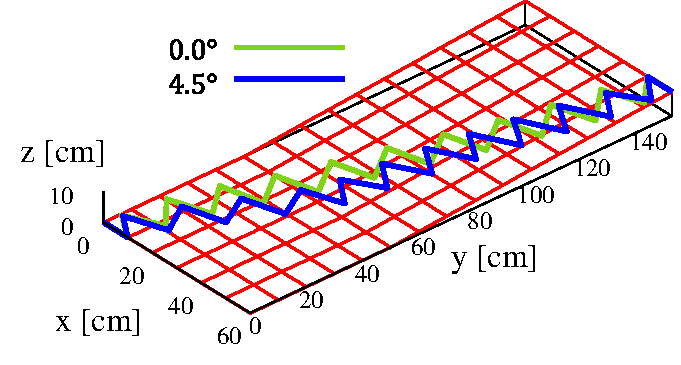
\includegraphics[width=\linewidth, clip]{./figure/sim_nao_slope_45_xyz.pdf}%
        \subcaption{x-y-z view}
        \label{fig:sim_nao_slope_45_xyz}%
    \end{subfigure}\\ %
    \begin{subfigure}[c]{0.6\linewidth}
        \centering%
        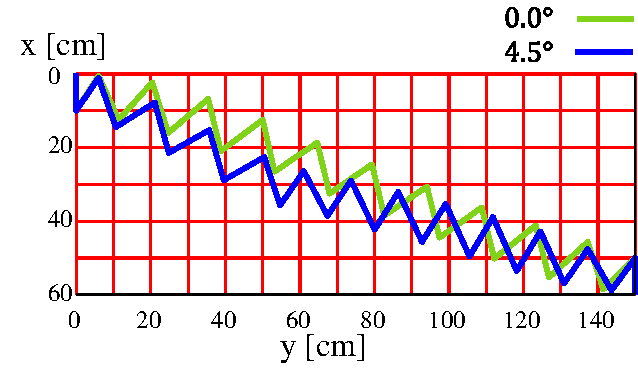
\includegraphics[width=\linewidth, clip]{./figure/sim_nao_slope_45_xy.pdf}%
        \subcaption{x-y view}
        \label{fig:sim_nao_slope_45_xy}%
    \end{subfigure}\\ %
    \begin{subfigure}[c]{0.5\linewidth}
        \centering%
        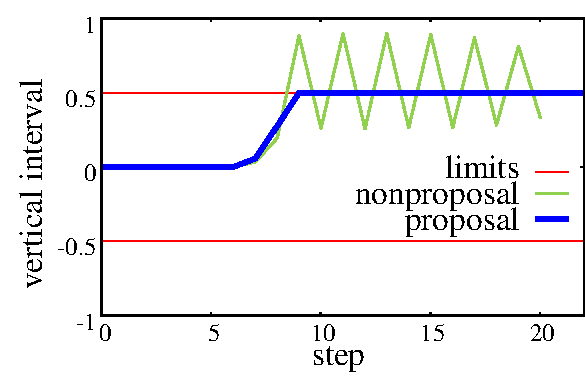
\includegraphics[width=\linewidth, clip]{./figure/sim_nao_slope_45_zdiff.pdf}%
        \subcaption{vertical interval}
        \label{fig:sim_nao_slope_45_zdiff}%
    \end{subfigure}%
    \caption{Footstep (slope)}%
    \label{fig:sim_nao_slope}%
\end{figure}

\section{スロープ型の地形でのシミュレーション}
\label{sec:sim_nao_slope}
初期状態$\bm{q}^0 = ( 0.0 ,\, 0.0 ,\, 0.0 ,\, 10.0 ,\, 0.0 ,\, 0.0 )^T\,(\cm ,\, \degrm)$から
目標状態$\bm{q}_{\goal} = ( 50.0 ,\, 150.0 ,\, 0.0 ,\, 10.0 ,\, 0.0 ,\, 0.0 )^T$へと向かう計画を行う.
地形としては,$y$軸方向において平面と傾斜角$\theta_{\slope}$の斜面が$y = 50\,\cm$の位置で接続しているスロープ型の地形を用いる.
\begin{equation}
    z_{\field}\left( x ,\, y \right) =
        \begin{cases}
            0.0 & \left( y < 50.0 \right) \\
            \left( y - 50.0 \right) \tan \theta_{\slope} & \left( 50.0 \leq y \right)
        \end{cases}
\end{equation}
$\theta = 0.0\degree$,$4.5\degree$の2パターンで計画を行う.


\Cref{fig:sim_nao_slope},\cref{tab:sim_nao_slope}に計画結果を示す.
$4.5\degree$の場合,平面上での歩幅に対して斜面上では歩幅を小さく取り,高低差制約を守りながら進む計画になっているのが
\cref{fig:sim_nao_slope_45_zdiff}からも分かる.
歩幅が狭いためステップ数は初期値から$1$増やす必要があり,また反復回数,計算時間は$0.0\degree$の場合に比べていずれも増加している.

\begin{table}[t]%
    \caption{Result of planning (slope)}%
    \label{tab:sim_nao_slope}%
    \centering%
    \begin{tabular}{ccccc}%
        \toprule%
        $\theta_{\slope}\,(\degrm)$ &   $k_{\init}$ &   $k$     &   iteration   &   time$(\ms)$ \\%
        \midrule%
        $0.0$                       &   $11$        &   $11$    &   $10$        &   $10.84$ \\%
        $4.5$                       &   $11$        &   $12$    &   $52$        &   $65.20$ \\%
        \bottomrule%
    \end{tabular}
\end{table}


\section{実地形データを用いた地形情報構築と計画}
実際のロボットが自律移動を行う場合,
環境の設計図などから事前に得られた地形形状を用いるのではなく,
環境中で測域センサなどを用いて計測したデータから適宜地形情報を構築し,
脚配置計画を行う必要がある.

ここでは,Kinect v2を用いて実際に取得した点群データから地形情報を構築し,
その地形データを用いて計画シミュレーションを行う.
\cref{sec:sim_nao_slope}と同様のスロープ型地形を用意し,
ワールド座標系基準で$(40.0 ,\, -113.0 ,\, 88.5)$の位置にチルト角$15.4\degree$で見下ろす姿勢で
設置したKinect v2で距離画像を取得する.
そして,取得した画像をワールド座標系基準の点群データへ変換し,それを用いて
\cref{sec:z_field_constructure}に示す手順で$z_\mathrm{field}(x ,\, y)$を構築する.
問題としても\cref{sec:sim_nao_slope}と同様,
初期状態$\bm{q}^0 = ( 0.0 ,\, 0.0 ,\, 0.0 ,\, 10.0 ,\, 0.0 ,\, 0.0 )^T\,(\cm ,\, \degrm)$から
目標状態$\bm{q}_{\goal} = ( 50.0 ,\, 150.0 ,\, 0.0 ,\, 10.0 ,\, 0.0 ,\, 0.0 )^T$へと向かう計画を行う.

\begin{figure}[t]%
    \centering
    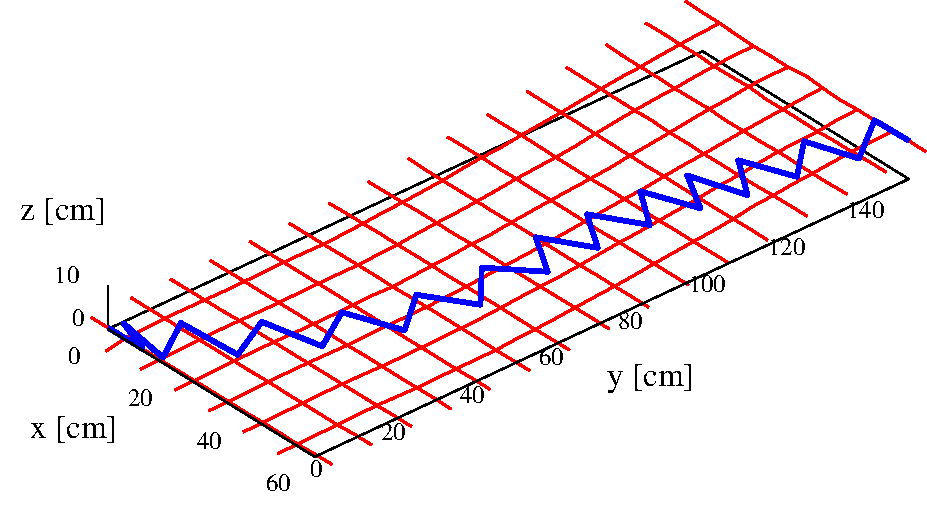
\includegraphics[width=0.8\linewidth, clip]{./figure/sim_nao_slope_45_kinect.pdf}%
    \caption{Footstep (slope mapped by using Kinect v2)}%
    \label{fig:sim_nao_slope_kinect}%
\end{figure}
\begin{table}[t]%
    \centering%
    \caption{Result of planning (slope using map data from Kinect v2)}%
    \label{tab:sim_nao_slope_kinect}%
    \begin{tabular}{ccccc}%
        \toprule%
        $\theta_{\slope}\,(\degrm)$ &   $k_{\init}$ &   $k$     &   iteration   &   time$(\ms)$ \\%
        \midrule%
        $4.5$                       &   $11$        &   $13$    &   $93$        &   $82.30$ \\%
        \bottomrule%
    \end{tabular}
\end{table}

\Cref{fig:sim_nao_slope_kinect}および\cref{tab:sim_nao_slope_kinect}に結果を示す.
ワンスキャンでの計測であること,およびノイズを考慮した地形情報構築が
できていないことなどから,マップに歪みが含まれている.
そのため,初期状態付近で地形適応制約を守るために
小さい歩幅で歩行する必要があり,
理想関数上での計画結果とは異なり$13$ステップでの計画となっている.
計算時間は十分歩行周期以内に収まっており,実時間制は保たれている.


\section{実機実験}
ここからは,実機を用いた実験について述べる.

NAOへの歩行指令では,まず脚配置計画を行い,得られた脚配置の系列から踏み出し量の系列を求める.
次に,NAOの制御システムであるNAOqi OSが標準で提供している,
踏み出し量と時間を指定して踏み出しを行わせるAPIを歩数分だけ呼び出して歩行を指令する.
このAPI呼び出しに対して,NAOqi OS内の歩行制御モジュールによって軌道生成が行われ,
指示した脚配置計画を実現する歩行制御が行われる.
なお,このAPIは平面上の歩行のためのものであり,平面上での位置と姿勢を指令するもので,
内部で行われる歩行制御も平面歩行のためのものである.
また,内蔵カメラの画像を用いた自己位置および姿勢の推定は行われておらず,
外部のカメラによる計測や補正も行っていない.


\subsection{計画の実機適用と動作確認}
まず,提案手法によって得られる脚配置計画が実際に実機に適用可能であることを確認する実験を行った.
\cref{sec:sim_nao_slope}におけるシミュレーションの傾斜角$4.5\degree$の場合の計画をNAOに適用した.
\Cref{fig:sim_nao_slope_45_exp}にその結果を示す.

\begin{figure}[t]
    \centering
    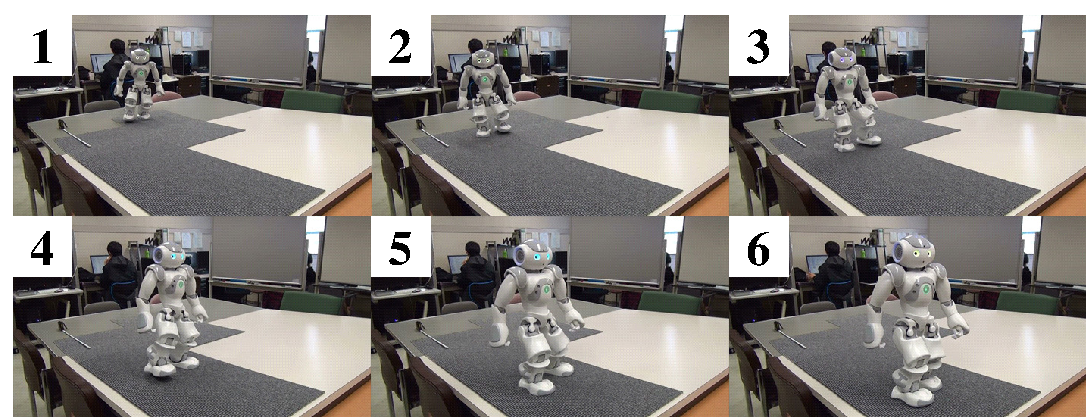
\includegraphics[width=1.0\linewidth, clip]{./figure/fig10.pdf}
    \caption{Experiment (slope)}
    \label{fig:sim_nao_slope_45_exp}
\end{figure}

平面上の歩行を仮定した歩行制御を用いて斜面を歩かせているため,
歩行が不安定になり姿勢が計画からずれたものとなった.
しかし,地形制約により上下方向の移動がNAOの許容値である$0.5\,\cm$以下に抑えられた計画がなされているため,
制御のロバスト性で姿勢を維持でき,目標状態付近まで到達することができている.
これにより,提案手法で実機に適用可能な脚配置計画が得られていることが確認できた.


\subsection{目標到達精度および歩行の安定性の評価}
次に,終了時の位置・姿勢と,歩行中の足裏圧力センサの値を計測し,
目標状態への到達精度と,歩行の安定性について評価する実験を行った.
いずれの評価においても,\cref{sec:sim_nao_slope}における傾斜角$4.5\degree$の場合の地形を対象とし,
提案手法による地形形状を考慮した計画と,
従来手法による平面上での計画の結果それぞれを用いて歩行させ,データを計測した.
なお,提案手法を用いない場合は$11$ステップの計画となっており,提案手法における計画結果の$12$ステップより少ない.

まず,目標状態への到達精度の評価について述べる.
歩行終了時の左脚の位置$x ,\, y$および姿勢$\theta$を計測し,
計画で設定した目標状態$(x = 50\,\cm ,\, y = 150\,\cm ,\, \theta = 0\degree)$に対する誤差を評価した.
なお,初期状態は$(x = 0\,\cm ,\, y = 0\,\cm ,\, \theta = 0\degree)$.
% 同様の計画を用いて平面上を歩行させた場合の位置・姿勢を真値として誤差を評価した.
提案手法,従来手法それぞれで五回ずつ実験を行った.
なお,NAOによる歩行精度の参考として,提案手法での計画を用いて平面上を歩かせた場合の歩行についても同様に計測を行った.
\cref{tab:result_goalerror}に,提案手法および従来手法での斜面歩行における誤差
および提案手法での平面歩行における誤差の,五回の試行での平均と標準偏差を示す.
\begin{table}[t]
    \caption{Results of evaluation experiment of goal reaching error}
    \label{tab:result_goalerror}
    \centering
    % \small
    \begin{tabular}{cccc}%
        \toprule%
        mathod              &   $x\,(\cm)$          &   $y\,(\cm)$      &   $\theta\,(\degrm)$ \\%
        \midrule%
        proposal            &   $-24.4 \pm  2.5$    &   $5.3 \pm 1.0$   &   $21.0 \pm 2.7$ \\%
        nonproposal         &   $-46.5 \pm 10.3$    &   $5.9 \pm 3.3$   &   $39.1 \pm 7.4$ \\%
        \cmidrule{1-4}%
        proposal (plane)    &   $ 2.3 \pm  3.7$     &   $6.7 \pm 1.6$   &   $5.4 \pm 2.8$ \\%
        \bottomrule%
    \end{tabular}
\end{table}
まず評価の前提として,提案手法で平面を歩行させた場合の結果からNAOによる歩行では平面上においても誤差が生じてしまうこと,
また提案手法での斜面歩行の結果と比較すると$x$,$\theta$について誤差が増加しており斜面歩行では更に精度が落ちることがわかる.
これを踏まえても,提案手法と従来手法とによる斜面歩行の結果を比較すると,
いずれの要素についても明らかに誤差が改善されており,特に$x$,$\theta$においては大きな改善が見られる.
標準偏差を比較しても,いずれの要素においても提案手法のほうが小さく抑えられている.
これらの結果から,従来手法に対して,提案手法によって目標到達の精度が改善されていることが分かる.

% 斜面上の計画を用いた場合の誤差に対する提案手法による改善率を評価した.
% 改善率は,$x$軸方向誤差については$17.4\,\%$,$y$軸方向誤差については$2.0\,\%$,
% 姿勢の誤差については$25.4\,\%$となり,提案手法によって斜面上での歩行精度が改善されていることがわかった.
% なお,平面上で歩行を行う場合であっても到達位置・姿勢に誤差が生じるため,
% 平面上で歩行させた場合の測定結果を斜面上の誤差データの基準とした.

% 提案手法,従来手法いずれにおいても,斜面上でのスリップなどで計画とのずれが生じ,
% 最終的な目標位置から大きくずれており,特に$x$軸方向および姿勢の誤差が大きくなっている.
% これらは平面上での歩行における誤差と比較しても明らかに大きい値となっている.
% しかしながら,平面上で歩行を行った場合の誤差を加味しても,
% 提案手法のほうが誤差を小さく抑えられていることがわかる.


\begin{figure}[t]%
    \centering%
    \begin{minipage}{0.49\linewidth}%
        \centering
        \begin{subfigure}[c]{\linewidth}
            \centering%
            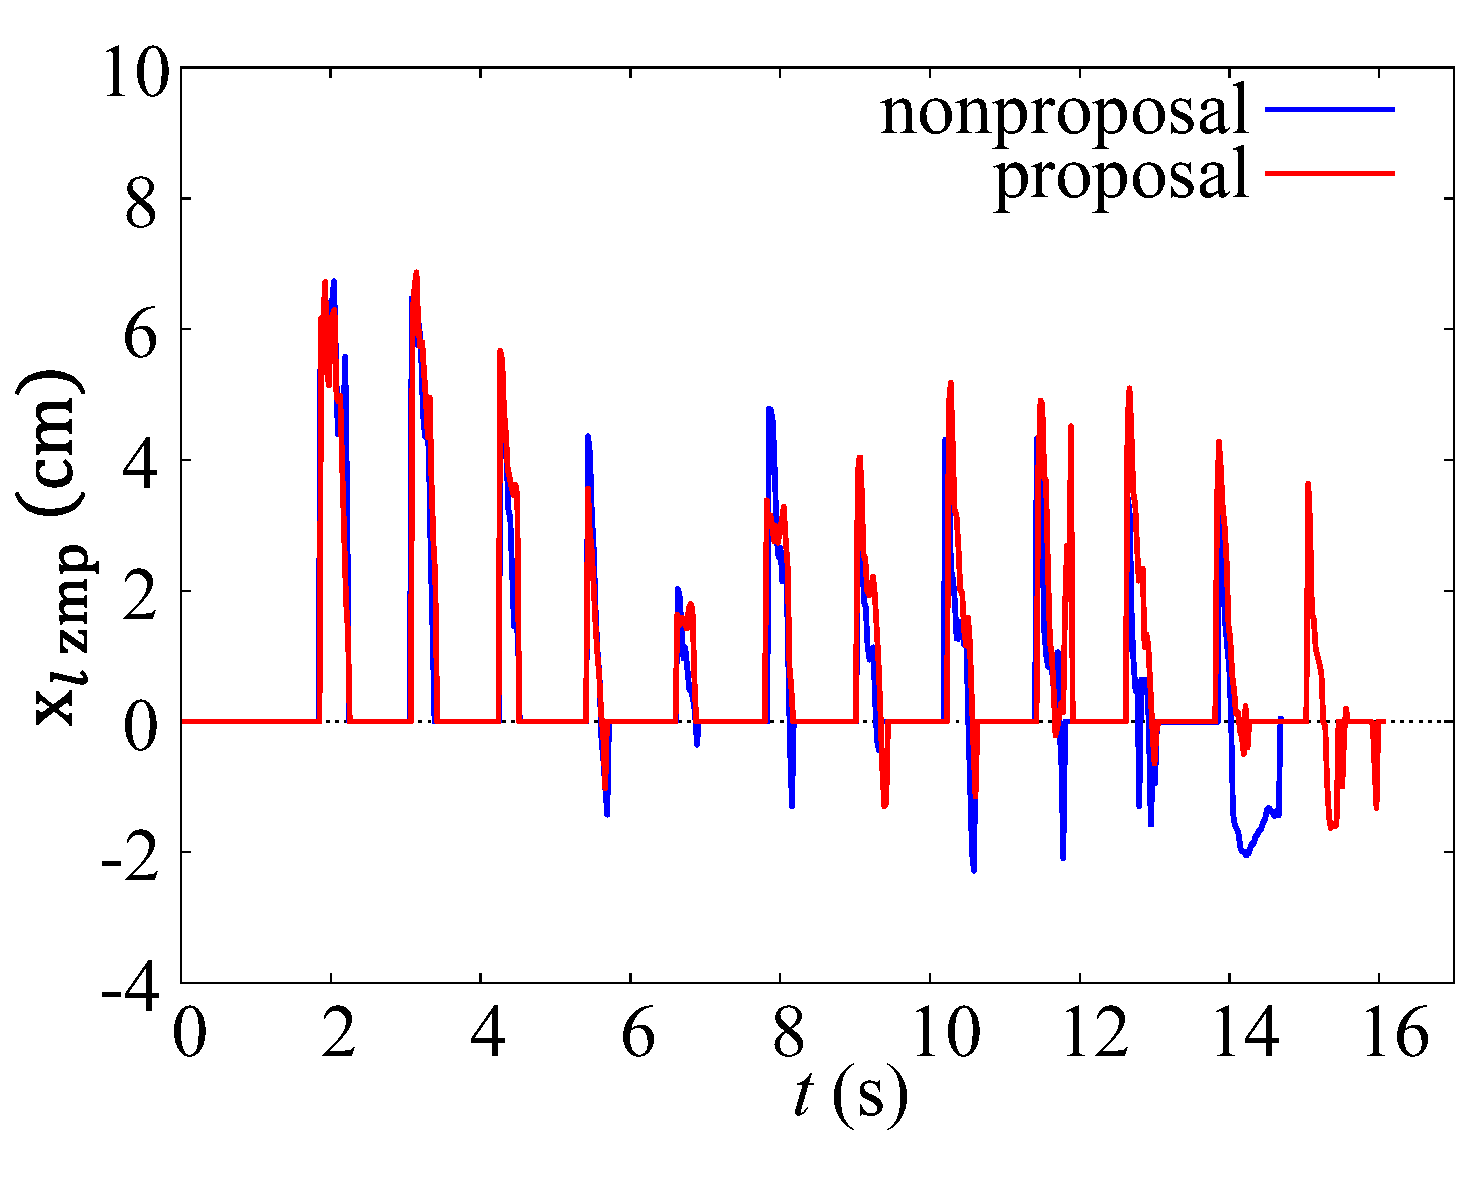
\includegraphics[width=\linewidth, clip]{./figure/fig11a.pdf}%
            \subcaption{left,$x$-axis}
            \label{fig:zmp_lx}%
        \end{subfigure}\\ %
        \begin{subfigure}[c]{\linewidth}
            \centering%
            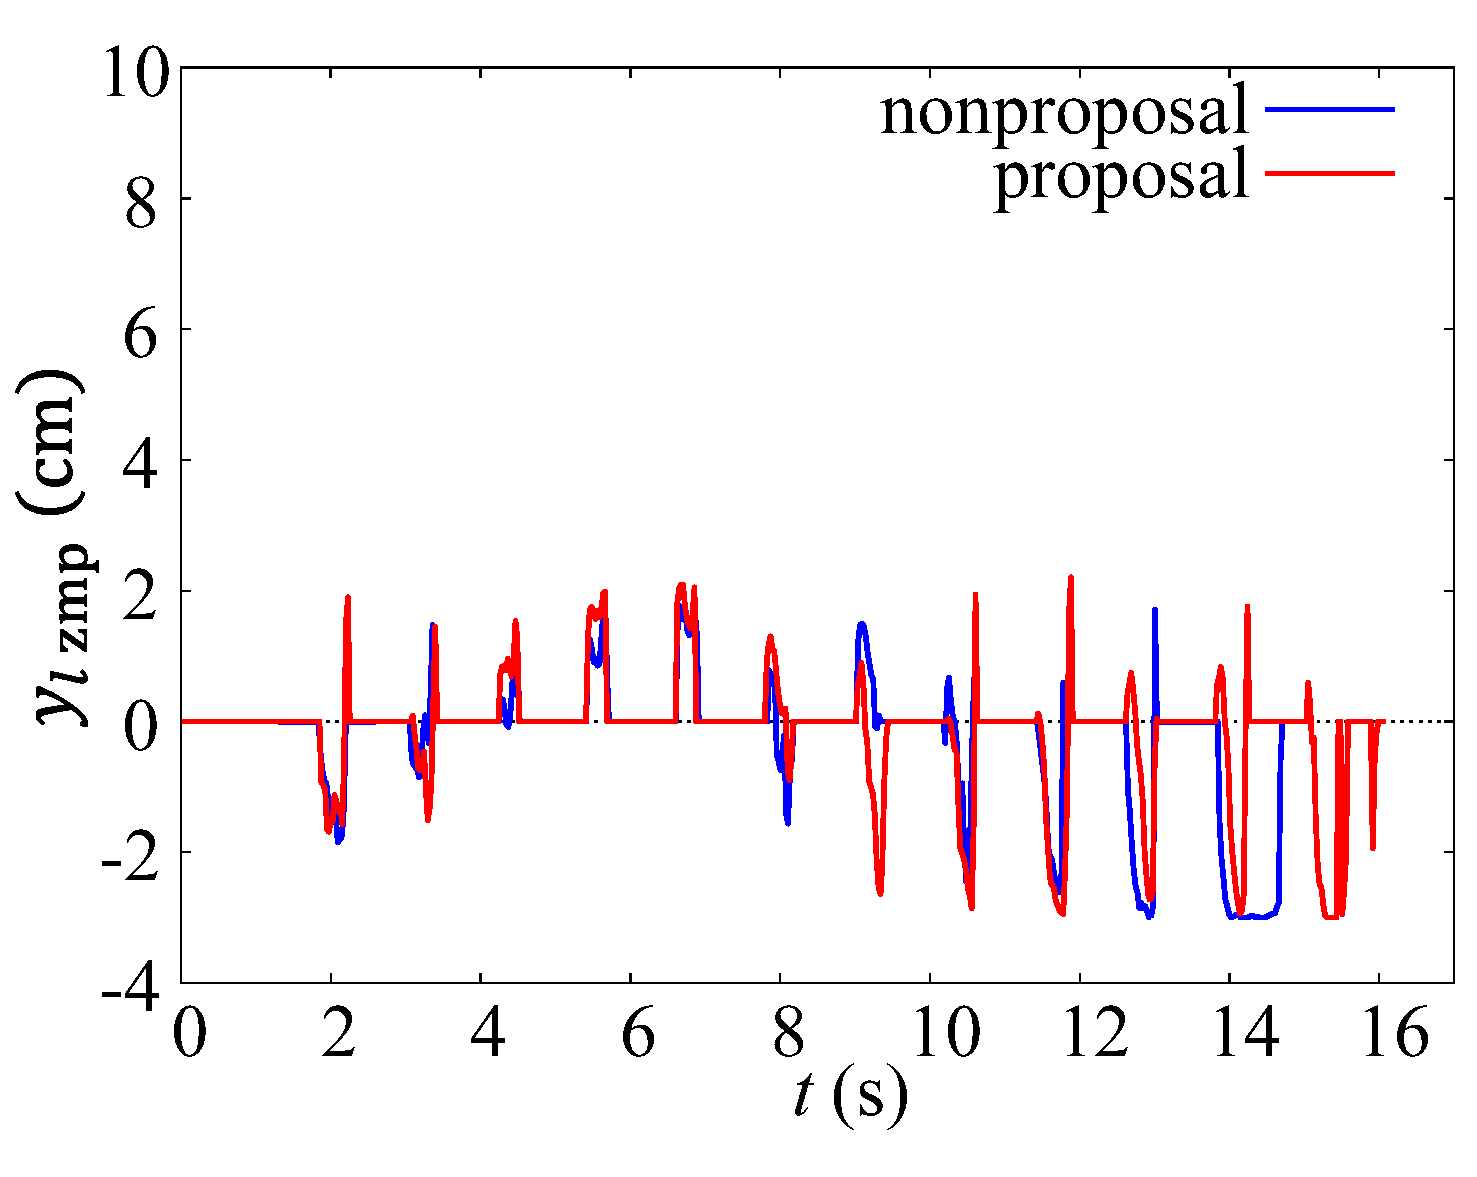
\includegraphics[width=\linewidth, clip]{./figure/fig11b.pdf}%
            \subcaption{left,$y$-axis}
            \label{fig:zmp_ly}%
        \end{subfigure}%
    \end{minipage}%
    \begin{minipage}{0.49\linewidth}%
        \centering
        \begin{subfigure}[c]{\linewidth}
            \centering%
            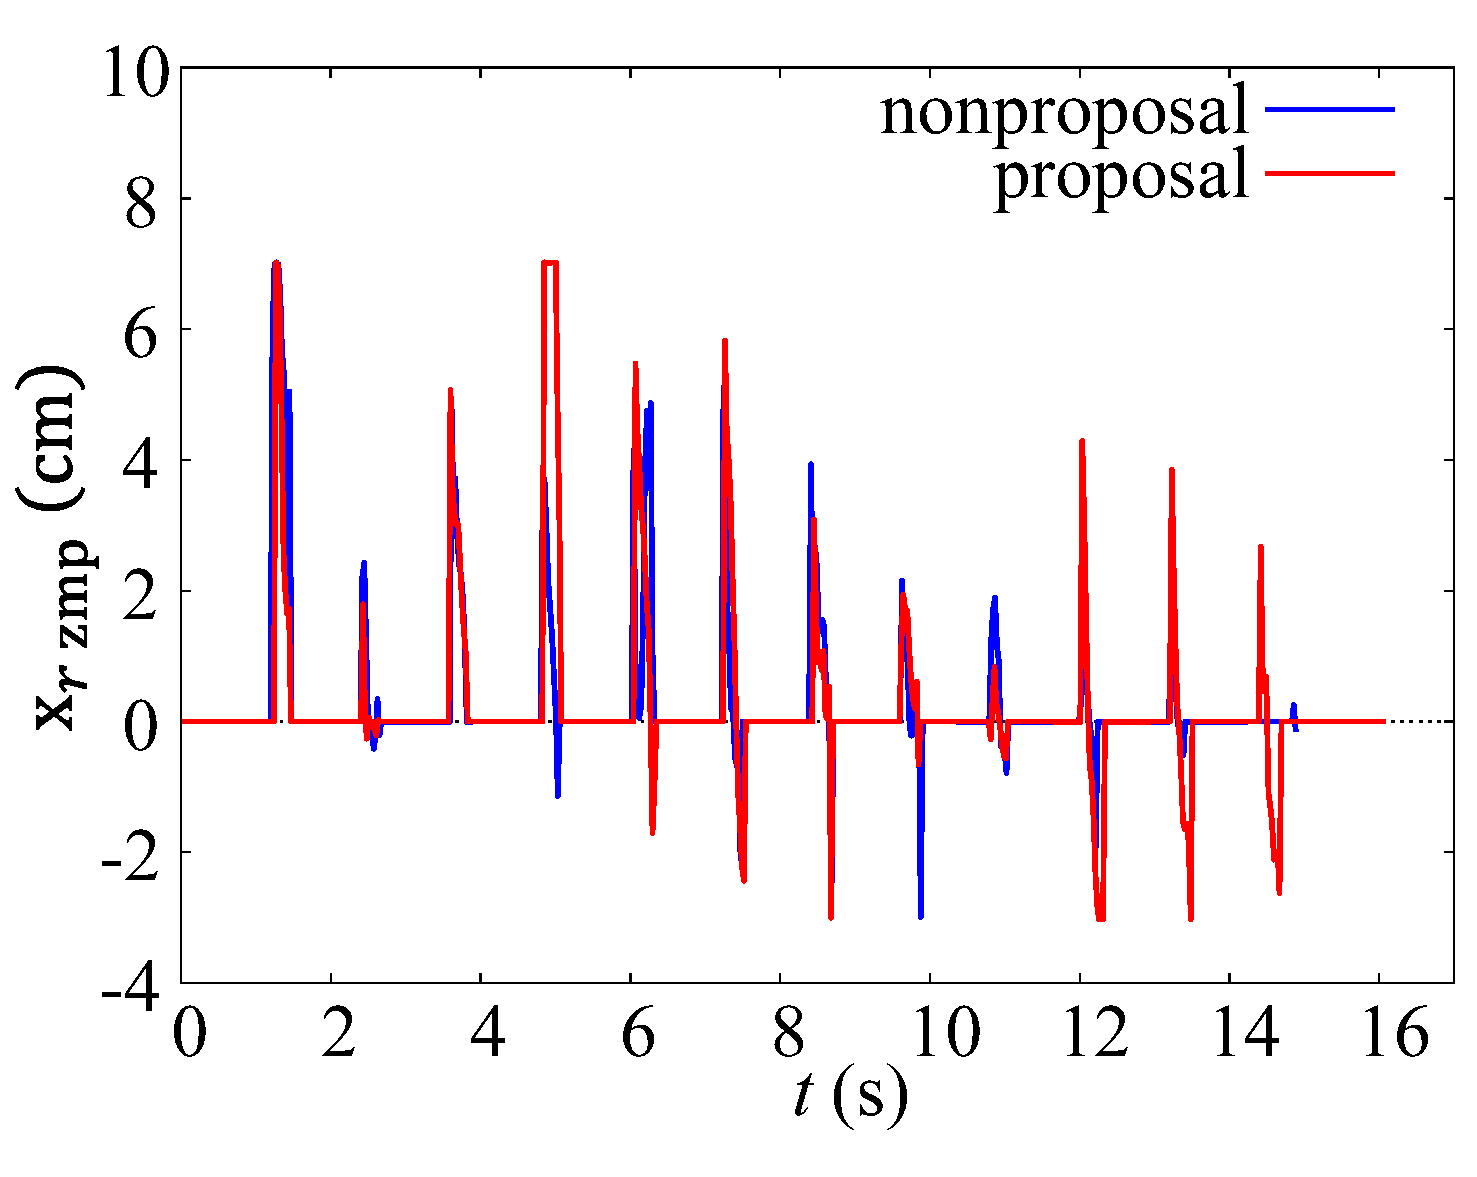
\includegraphics[width=\linewidth, clip]{./figure/fig11c.pdf}%
            \subcaption{right,$x$-axis}
            \label{fig:zmp_rx}%
        \end{subfigure}\\ %
        \begin{subfigure}[c]{\linewidth}
            \centering%
            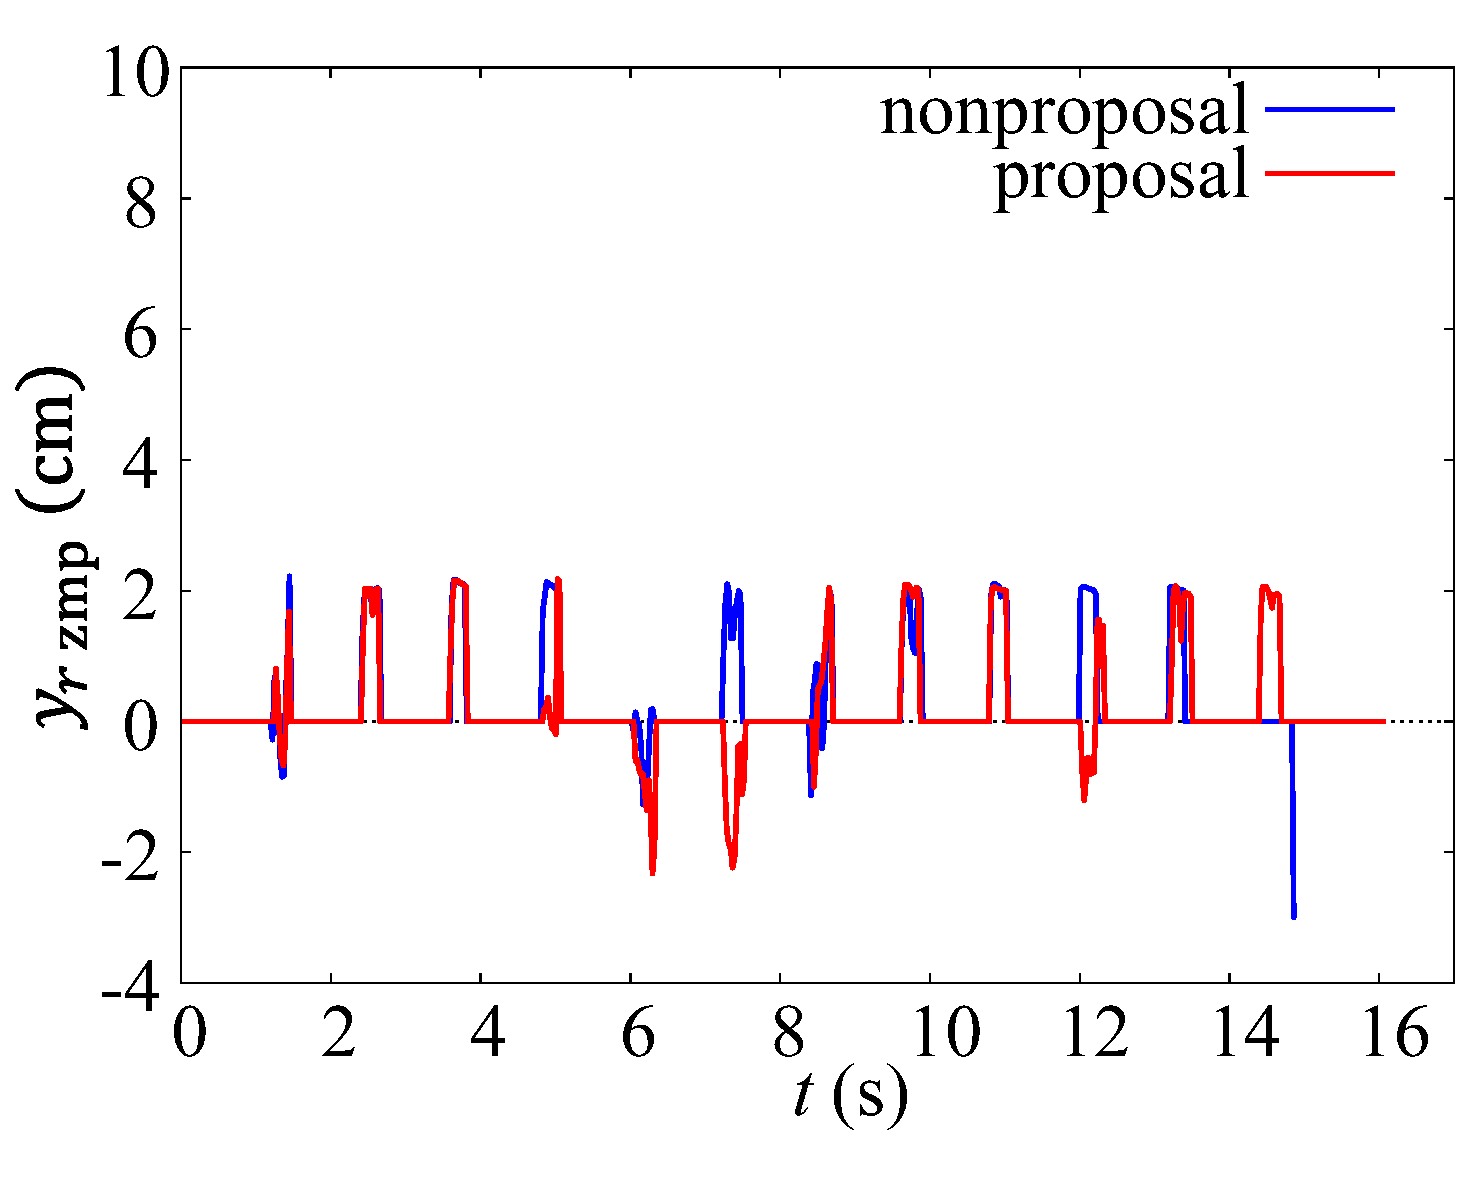
\includegraphics[width=\linewidth, clip]{./figure/fig11d.pdf}%
            \subcaption{right,$y$-axis}
            \label{fig:zmp_ry}%
        \end{subfigure}%
    \end{minipage}%
    \caption{ZMP values in the single support phase}%
    \label{fig:zmp}%
\end{figure}

次に,片脚支持期のZMP値を用いた歩行の安定性の評価について述べる.
NAOの左右の足裏それぞれ四ヶ所($(7.025, 2.310)$,$(7.025, -2.990)$,$(-3.025, 1.910)$,$(-2.965, -2.990)$($\cm$))に
配置されている圧力センサの値を$25\,\ms$ごとに計測し,
脚先座標系$\Sigma_{fl}$および$\Sigma_{fr}$基準の片脚支持期のZMP応答値を算出した.
\Cref{fig:zmp}に提案手法および従来手法それぞれにおける左右の$x$,$y$軸方向のZMP応答値を示す.
% \begin{figure*}[t]%
%     \centering%
%     \subfigure[left,$x$-axis]{%
%         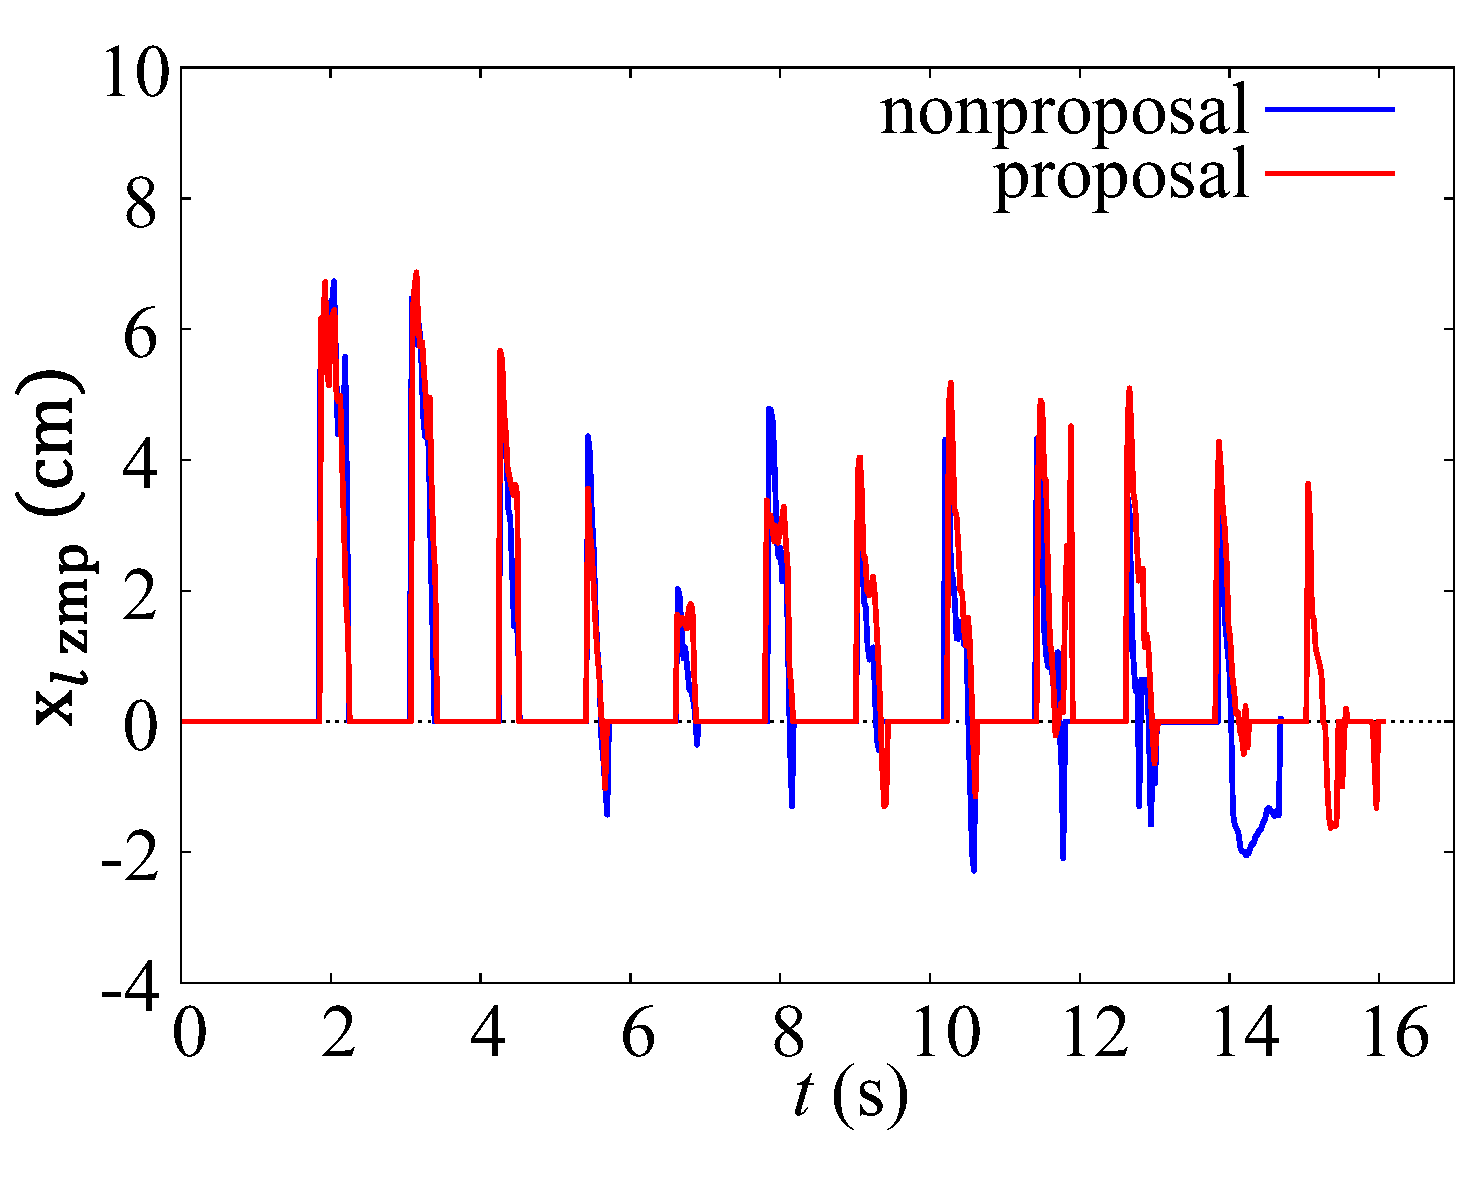
\includegraphics[width=0.25\linewidth, clip]{./figure/fig11a.pdf}%
%         \label{fig:zmp_lx}}%
%     \subfigure[left,$y$-axis]{%
%         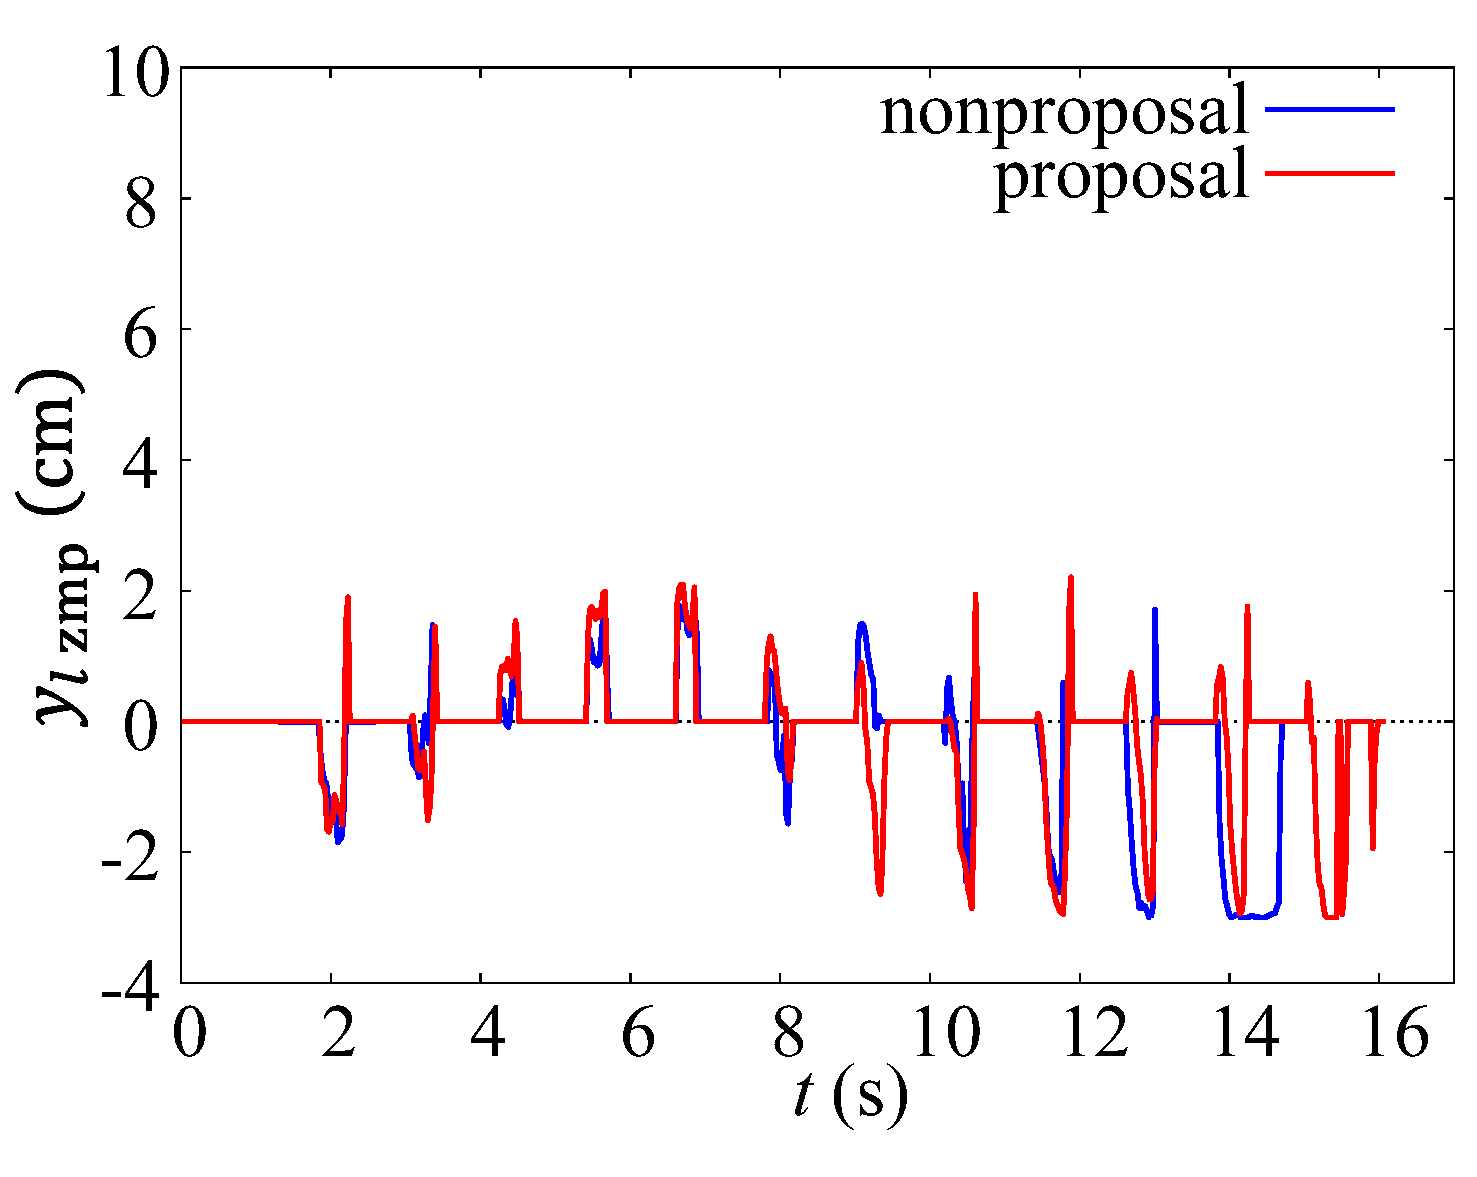
\includegraphics[width=0.25\linewidth, clip]{./figure/fig11b.pdf}%
%         \label{fig:zmp_ly}}%
%     \subfigure[right,$x$-axis]{%
%         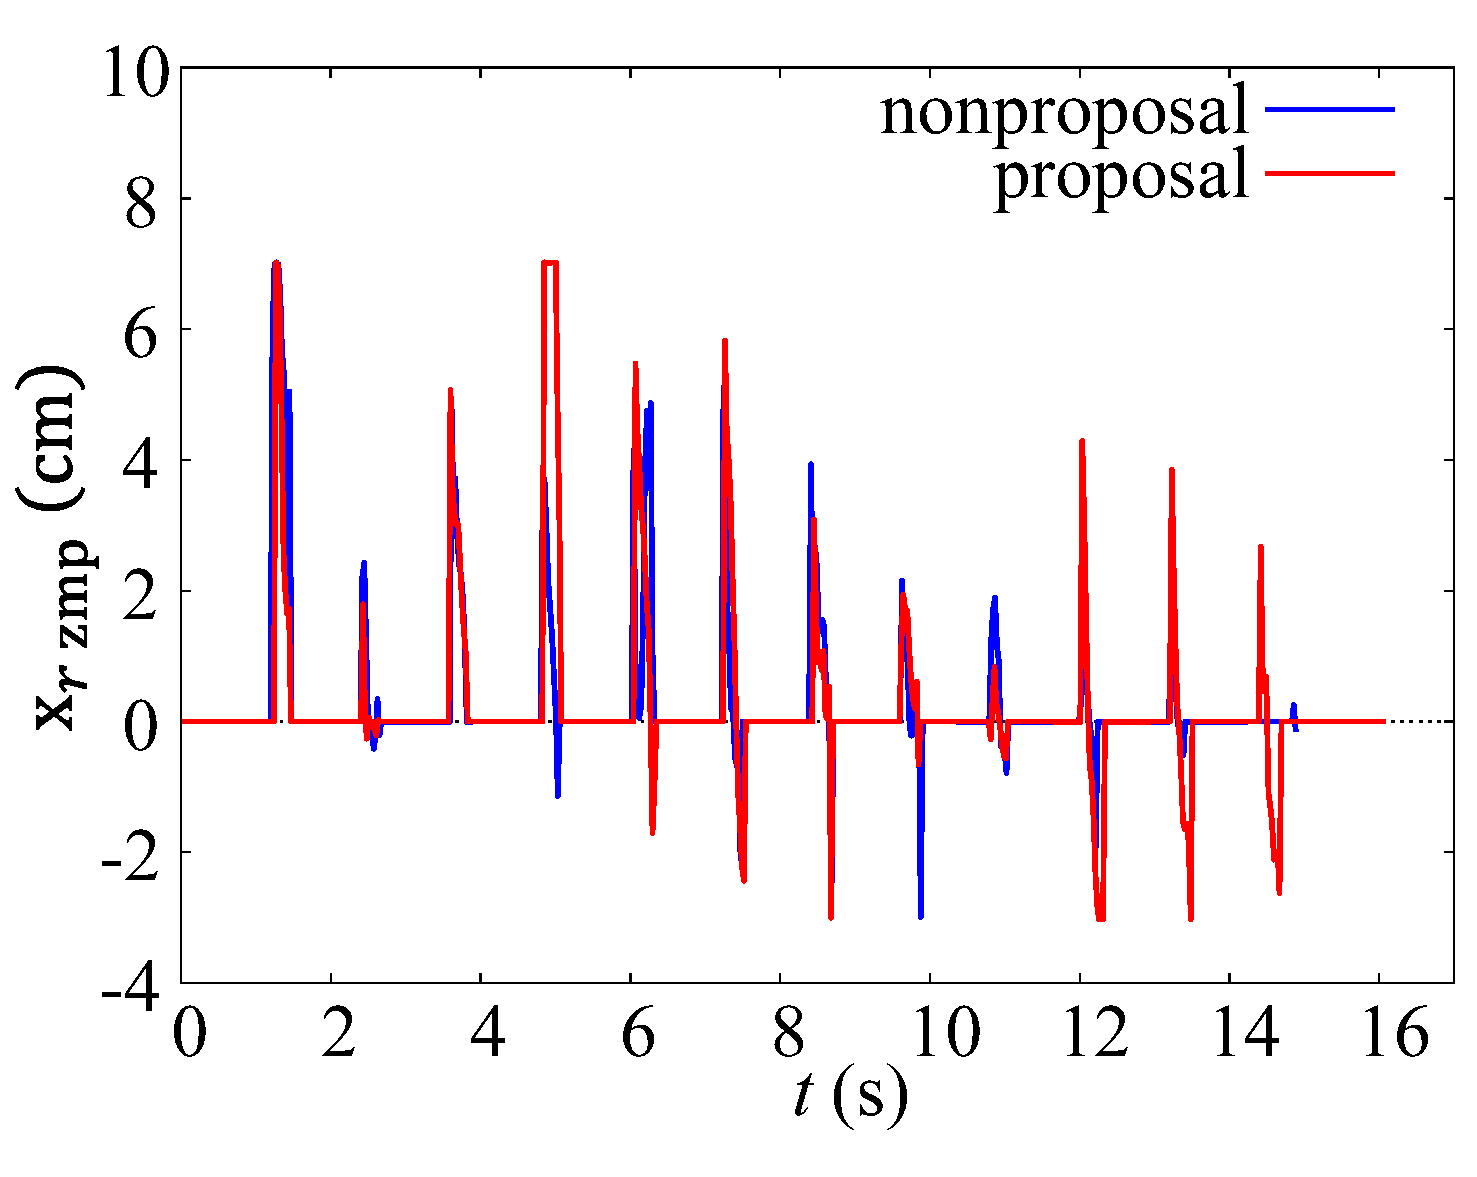
\includegraphics[width=0.25\linewidth, clip]{./figure/fig11c.pdf}%
%         \label{fig:zmp_rx}}%
%     \subfigure[right,$y$-axis]{%
%         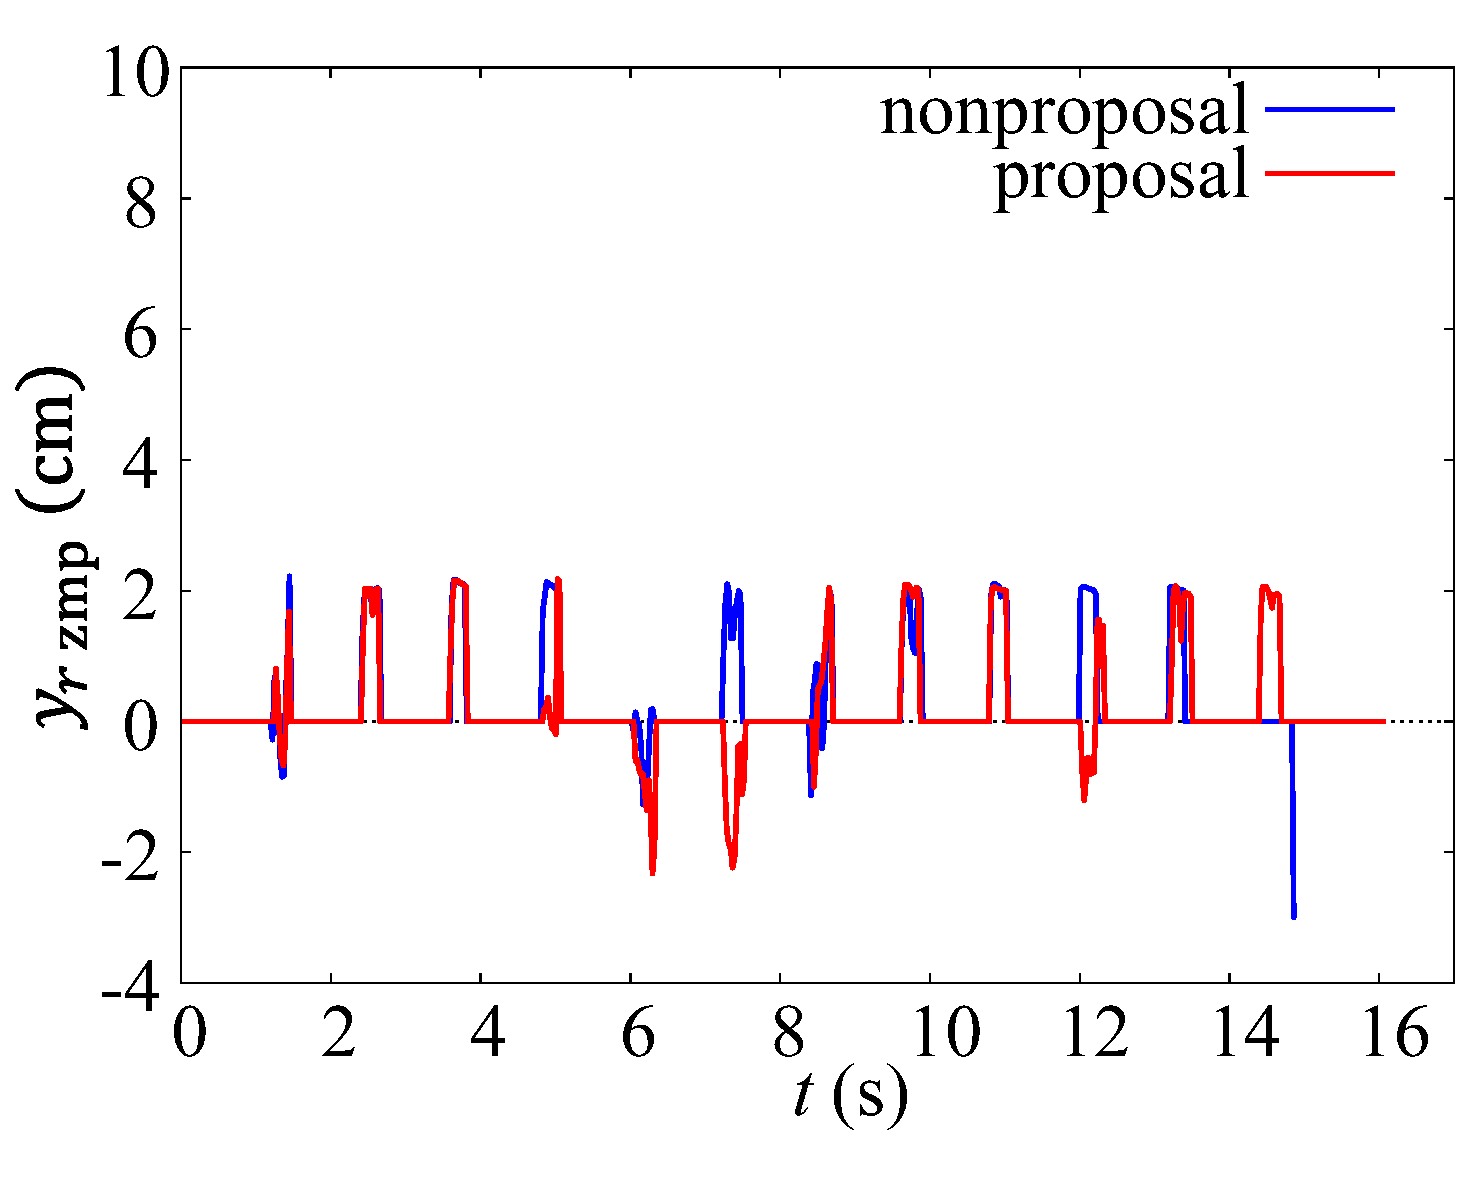
\includegraphics[width=0.25\linewidth, clip]{./figure/fig11d.pdf}%
%         \label{fig:zmp_ry}}%
%     \vspace*{-5pt}%
%     \caption{ZMP values in the single support phase}%
%     \label{fig:zmp}%
%     \vspace*{-10pt}%
% \end{figure*}
提案手法と従来手法とで$12\,\mathrm{s}$以降の左脚のZMP応答を比較する.
$x$軸方向\cref{fig:zmp_lx}及び$y$軸方向\cref{fig:zmp_ly}いずれについても,
従来手法においては,本来$12\,\mathrm{s}$以前の応答と同様にすぐに$0$に戻るはずであるが,
$0$から変化したあとに戻るのが明らかに遅く,歩行が不安定になっていることが分かる.
提案手法ではこのようなZMPの応答は見られず,それ以前と同様の応答を示しており,
斜面上においても安定して歩行ができていることが分かる.

% 従来手法および提案手法どちらにおいても,斜面上の歩行で支持期間中にZMPの符号が反転するなどしており,
% 提案手法における優位性は見られなかった.
% これは,どちらの計画においても,\cref{sec:simulation}で述べたとおり
% 平面歩行の制御で斜面を歩いていることに変わりはないからであると考えられる.

最後に,床反力の評価について述べる.
ZMP評価と同様に三回目の実験データを用い,左右それぞれについて圧力センサの示す値の合計値を比較した.
一つの圧力センサで最大$25 \,\mathrm{N}$まで計測でき,片脚全体の床反力は最大$100 \,\mathrm{N}$である.
\Cref{fig:force}に提案手法および従来手法それぞれにおける左右の足裏の床反力の遷移を示す.
\begin{figure}[t]
    \centering
    \begin{subfigure}[c]{0.50\linewidth}
        \centering%
        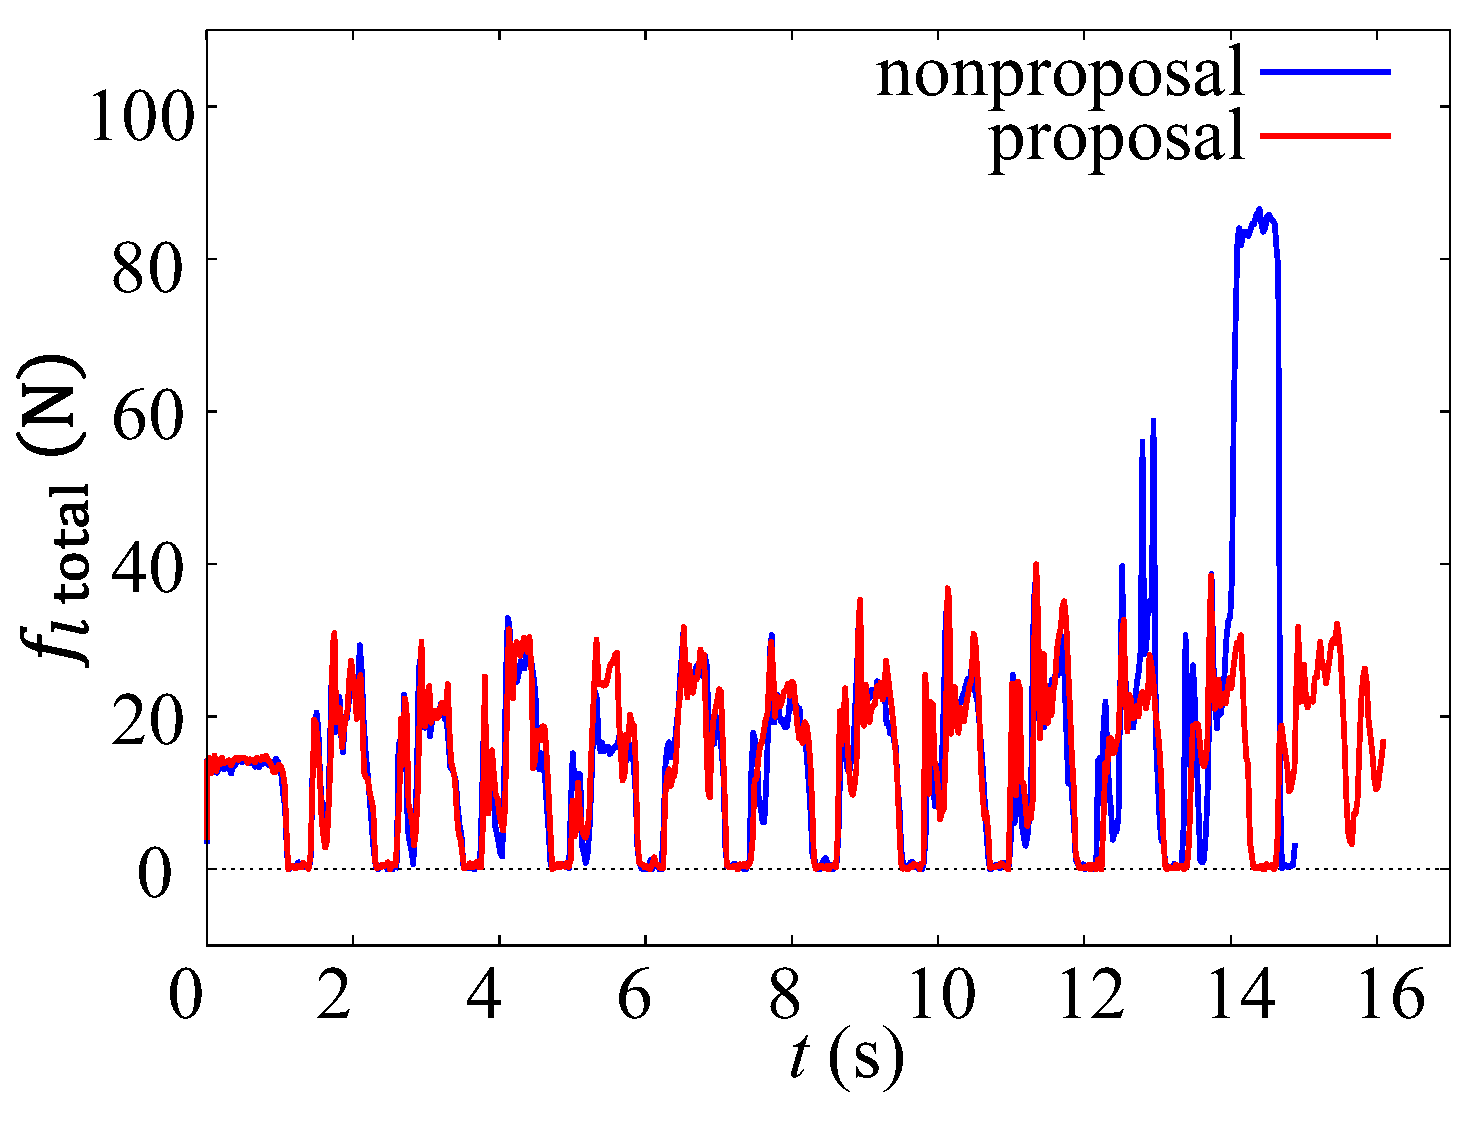
\includegraphics[width=\linewidth, clip]{./figure/fig12a.pdf}%
        \subcaption{left}
        \label{fig:fl_total}%
    \end{subfigure}%
    \begin{subfigure}[c]{0.5\linewidth}
        \centering%
        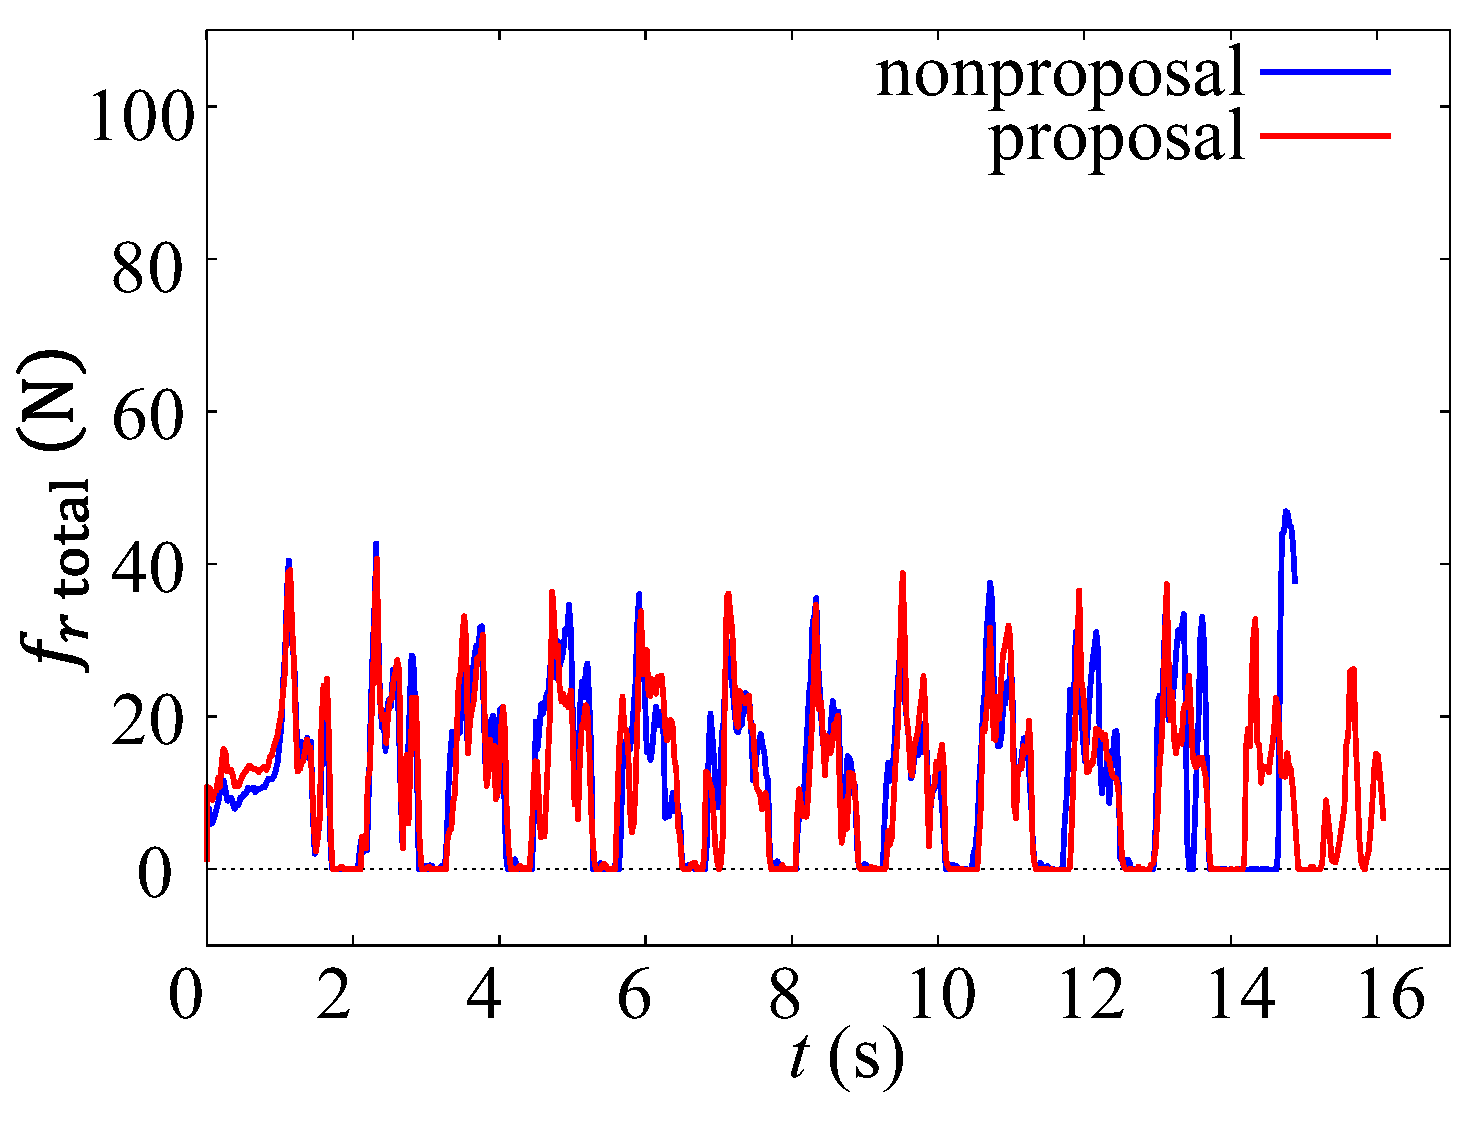
\includegraphics[width=\linewidth, clip]{./figure/fig12b.pdf}%
        \subcaption{right}
        \label{fig:fr_total}%
    \end{subfigure}%
    \caption{Ground reaction force}%
    \label{fig:force}%
\end{figure}
提案手法を用いない場合の結果において,左脚の床反力値が$12\,\mathrm{s}$以降に高い値をとっている.
これはバランスを崩したことによって左脚が強く着地してしまったことを表しており,
歩行が不安定になっていたと考えられる.
これに対して,提案手法では床反力は最後まで周期的に変化しており,
歩行の安定性が改善されていると言える.

以上の実験データおよび評価から,目標到達精度,
およびZMP応答および床反力で評価した歩行の安定性ついて
提案手法の有効性が確認された.


\section{本章のまとめ}
本章では,二足歩行ロボットNAOにおいて,
標準の平面歩行制御における垂直方向のロバスト性を利用した三次元地形での計画として,
まず,計画シミュレーションによりスロープ形状の地形に適応した脚配置計画が得られることを確認した.
また,Kinect v2センサを用いて実際に計測したスロープに対しても同様に計画ができることを示した.
さらに,実機実験により実際に前述のロバスト性を利用してスロープを歩行できる
計画が得られていることや,目標到達の精度や歩行の安定性について有効性があることを示した.


\end{document}
